\section{Experimental Results}
\label{sec:eval}
In this section, we first give some statistics of our corpus and the
extracted causal network, and then evaluate the quantity
and quality of the cue patterns used in the extraction.
We further compared the end-to-end results on COPA task with
several previously published results.
Finally, we evaluate our commonsense reasoning ability on
two additional tasks using data from ConceptNet 4 to further
showcase the power of our framework. A demo of our network
as well as the test sets we used in this section at
\url{http://202.120.38.146/causal}.
%This section presets our training setting and
%show our results for two tasks.

\subsection{Data Set and Extraction of Causal Network}
\begin{figure}[th]
\centering
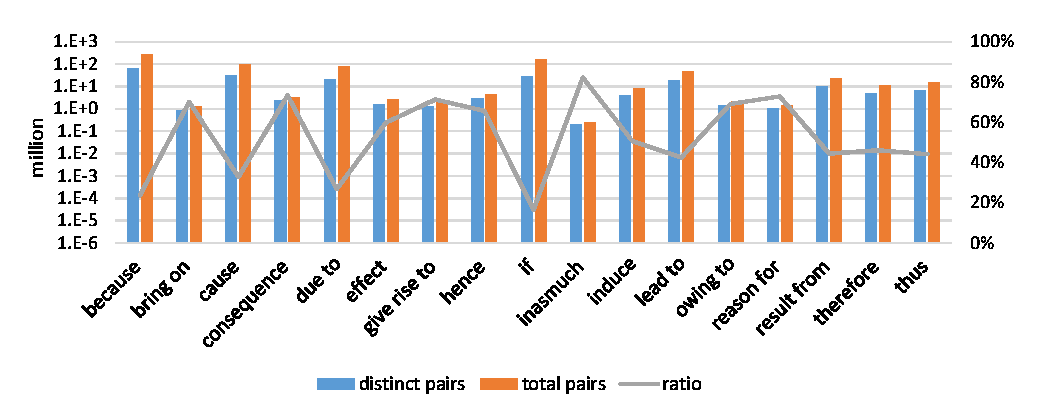
\epsfig{file=pattern1.eps, width=\columnwidth}
%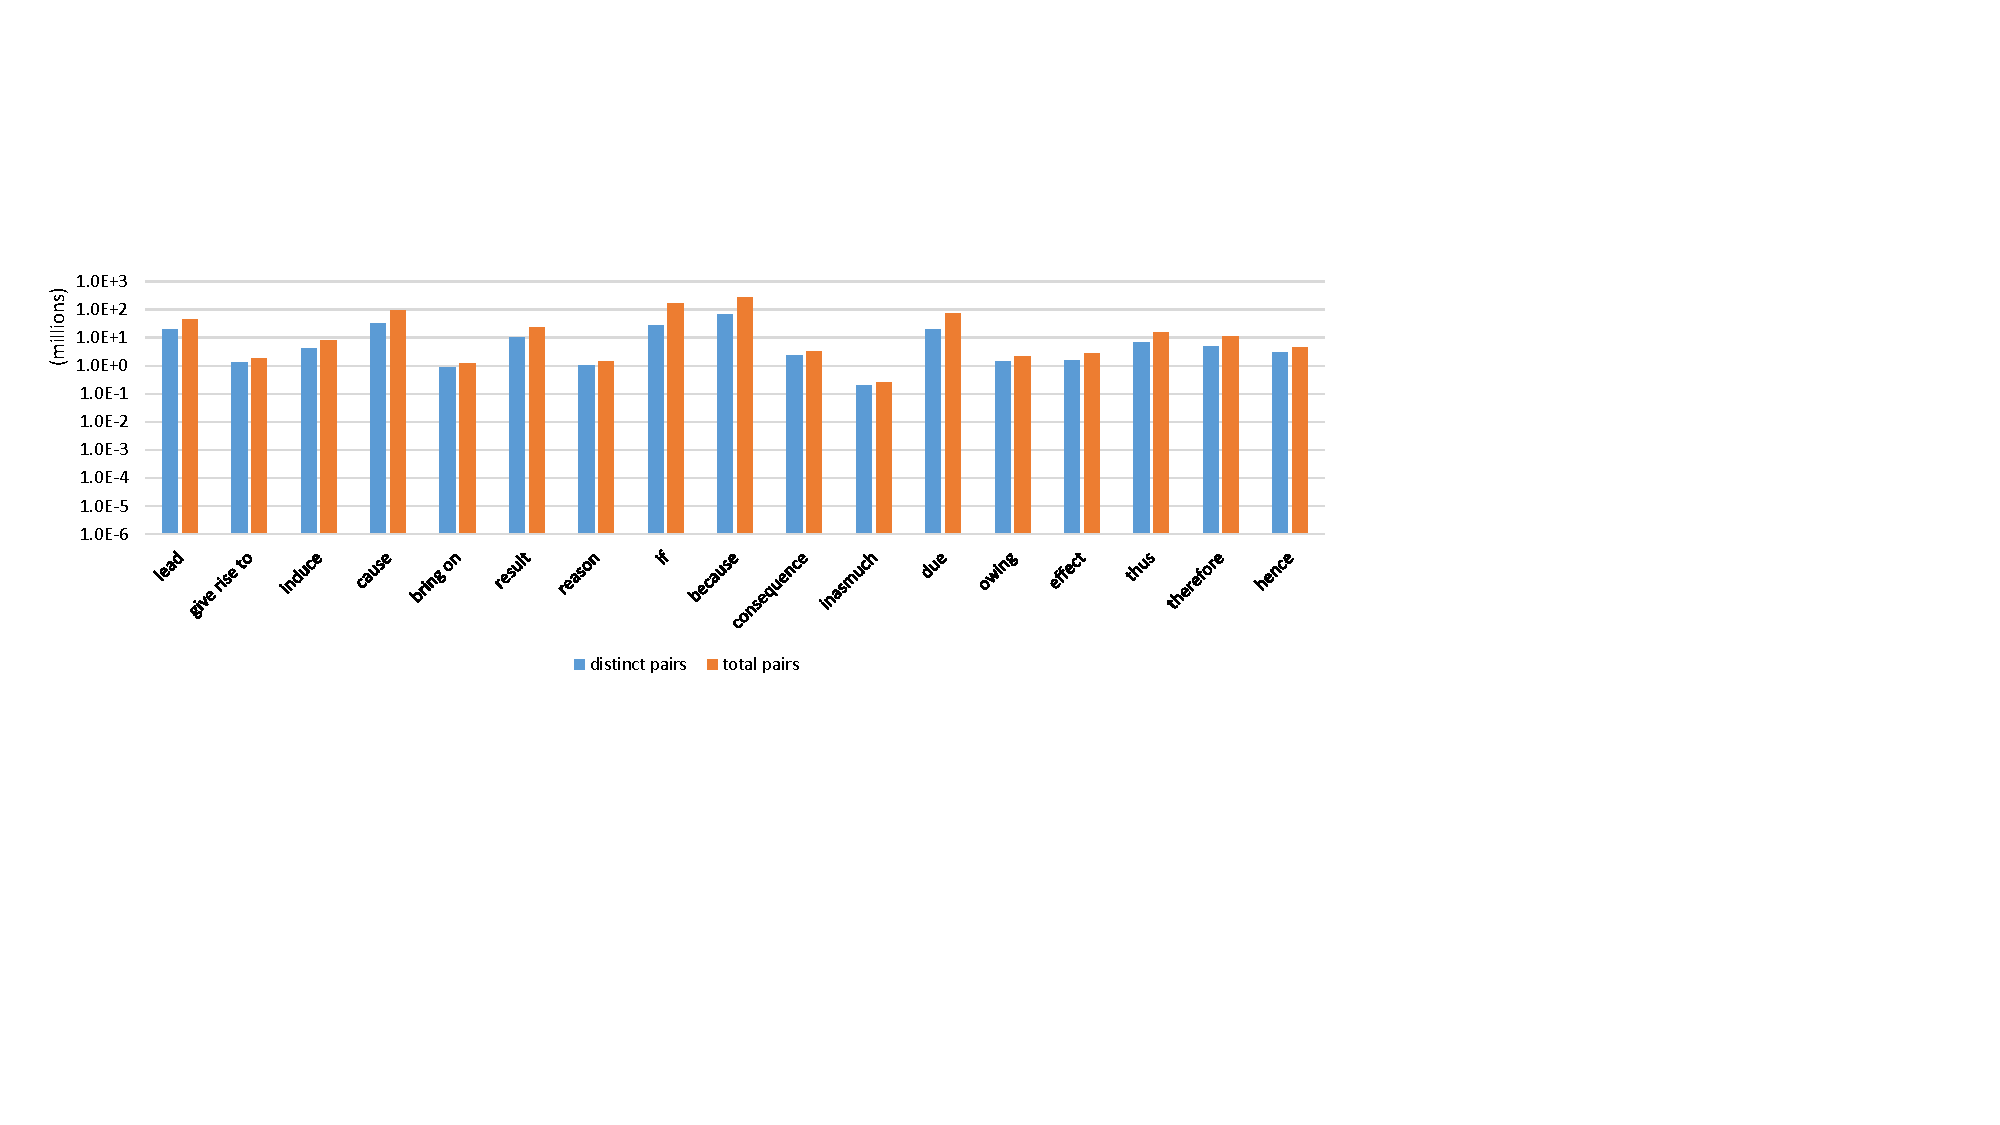
\includegraphics[width=2\columnwidth]{pattern.pdf}
\caption{Number of (distinct) pairs extracted by Cues}
\label{fig:pattern1}
\end{figure}
We extracted our term causality network, which we call ``CausalNet''
for convenience in this section, from 1/10
of a commercial search engine web snapshot~\footnote{Anonymized to
honor double blind policy}.
The snapshot was generated in February, 2013 and contains about 1.6
billion web pages with a combined of nearly 10TB.
We extract 68,217,404 distinct word pairs from this corpus, 
which amounts to roughly 8GB. The number of unique lemmatized words in 
these pairs is 64,436, covering 41.49\% (64,436/155,287) of the 
words in WordNet. 

The 53 causal cues we used can be grouped into 17 sets, each
containing cues of the same meaning or lemma form but with different
tenses. Word pair distribution over these sets is shown in Figure
\ref{fig:pattern1}. The blue bars (left) are the number of distinct
pairs and the orange one (right) show the total number of pairs.
Inter-sentence cues like ``if'' and ``because'' harvested the
largest number of pairs. But more specific patterns such as
``reason'' and ``inasmuch'' find more diverse pairs, since the
number of distinct pairs is relatively large compared to the total
pairs extracted.

\begin{figure}[th]
\centering
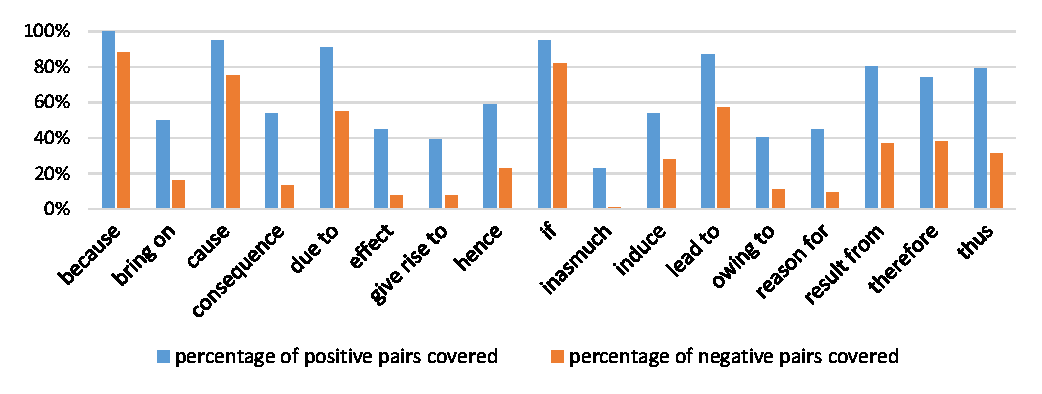
\epsfig{file=pattern3.eps, width=\columnwidth}
%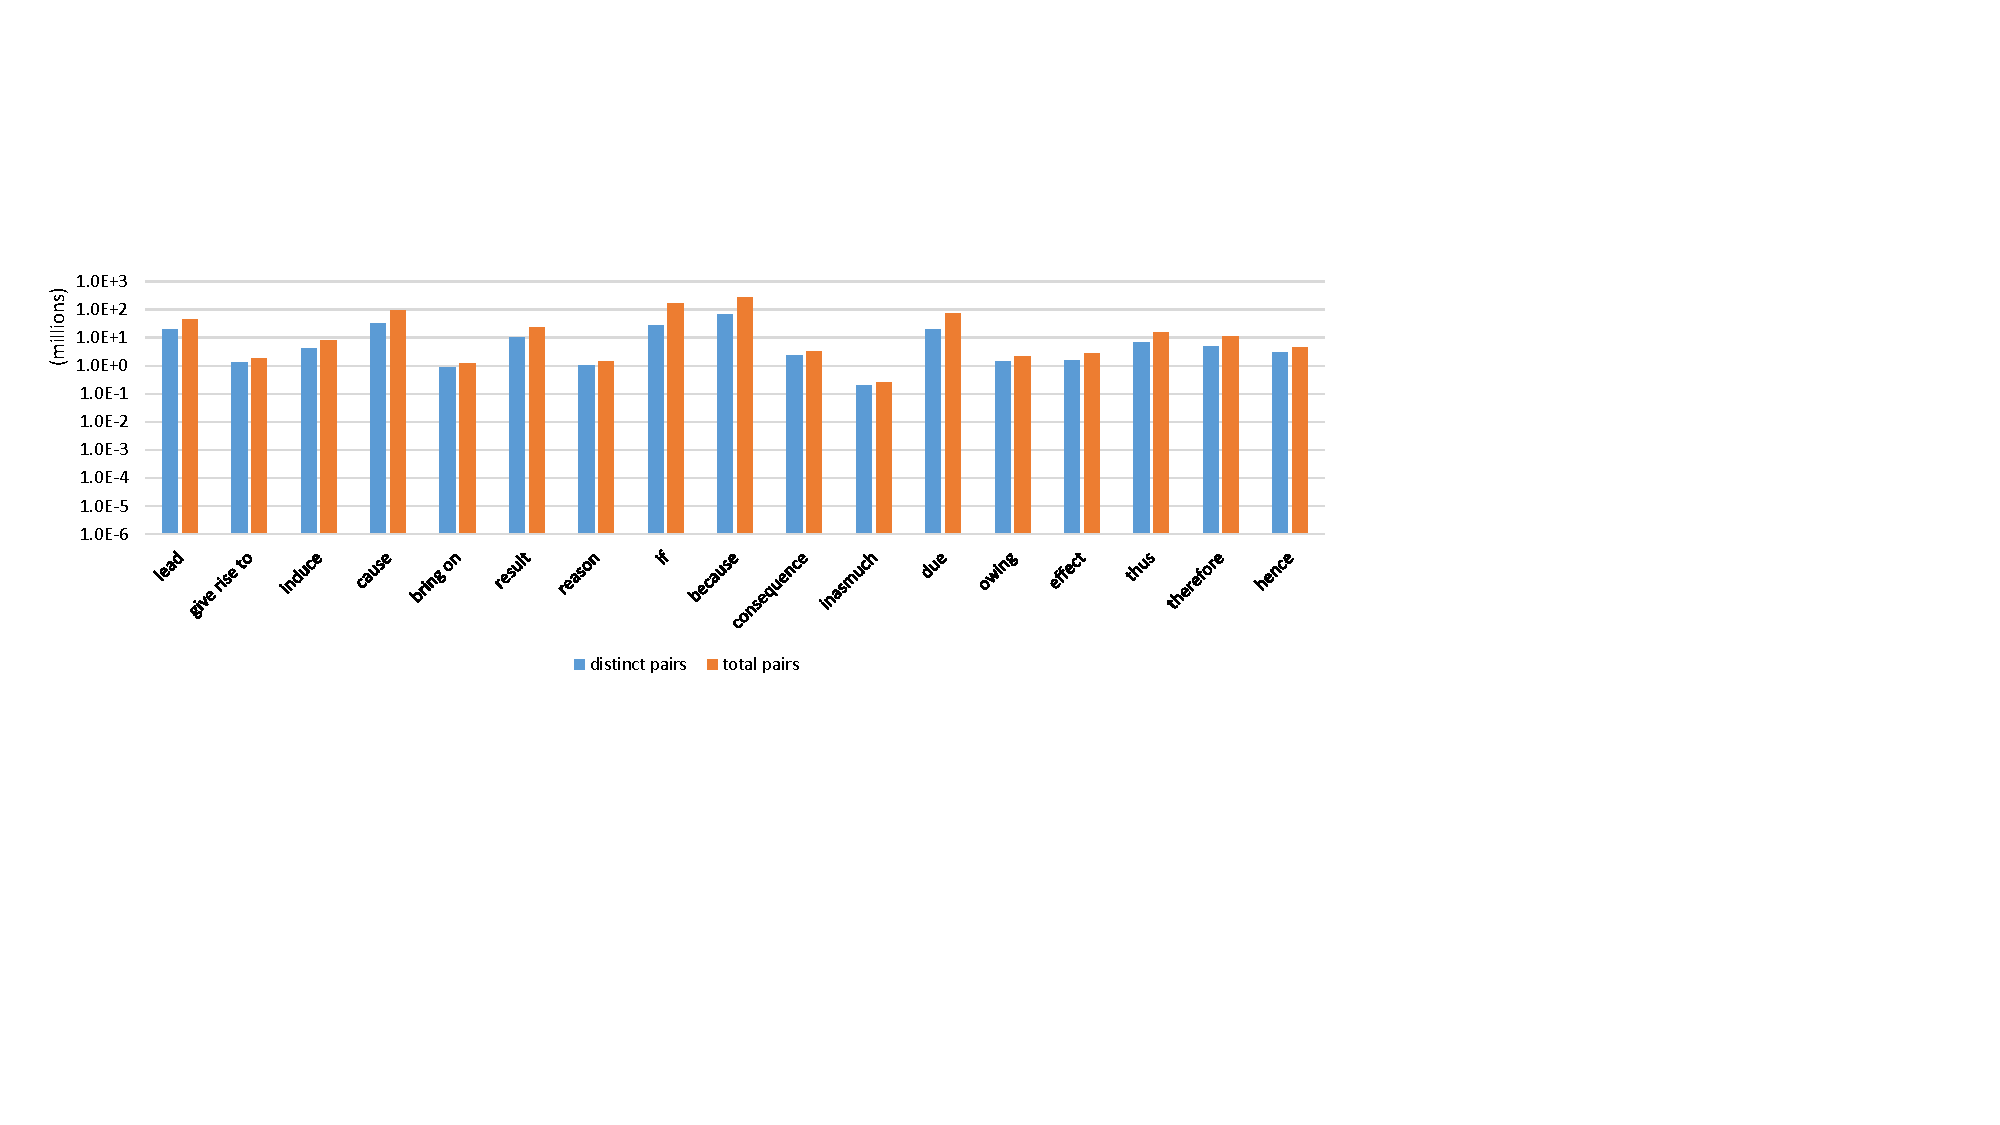
\includegraphics[width=2\columnwidth]{pattern.pdf}
\caption{Positive vs. negative ConceptNet causal pairs covered by cues}
\label{fig:pattern2}
\end{figure}

To evaluate the quality of the causal cues, we make use of the
manually labeled causal events in
ConceptNet~\cite{liu2004commonsense} as ground truth. ConceptNet 4
contains 74,336 unlemmatized English words, forming
375,135 unique concepts, which are connected by 610,397 relations.
It is significantly smaller than our CausalNet in scale, 
especially in terms of number of edges. In otherwise, relations are
more sparse in ConceptNet.
We randomly collect 100 positive and 100 negative causal event pairs, 
based on feedbacks from human volunteers of OMCS project, casting positive
votes for each \emph{Causes} relationship that is causal, and
negative for that is not. Since the pairs from ConceptNet contain
phrases and not just words, we consider a pair is covered by a
causal cue, if it extracted at least one pair of words from the web
corpus, where the cause word appears in the cause event and effect
word appears in the effect event in the ConceptNet pairs.
\figref{fig:pattern2} shows that in general, our cues can
effectively distinguish between positive and negative causal pairs,
with the exception of ``hence'' and ``consequence'', both of which
represent relatively coarse-grained entailment relation.
Particularly good cues to distinguish the positive and negative
pairs are ``due'' and ``induce''.

\subsection{End-to-end Evaluation on COPA}
COPA task consists of 1000 causal reasoning questions, divided into 
development question set and test question set of 500 each.
We pruned the parameter $\alpha$ and $\beta$ on the development set
by attempting all combinations of values
from  0.1 to 1.0 with a step of 0.1. The best combination turns out to be
$\alpha=0.4$, $\beta=0.3$.
All competing systems were assessed based on their
accuracy on the 500 questions in the COPA test split \cite{gordon2012copa}. 

%but we also show the accuracy on development set and all questions.
%The overall score is the mean value of development and test set because the two
% sets have equal number of examples.
\tabref{tab:evaluation} shows the results.
%Table~\ref{tab:evaluation} 


%\begin{table}[th]
%\small
%\centering
%\caption{COPA results comparison}
%\begin{tabular}{|l|c|c|c|}
%\hline Methods & Dev & Test & All  \\ \hline \hline
%PMI Gutenberg (W=5)\cite{roemmele2011choice} & 57.8\% & 58.8\% & 58.3\% \\
%UTDHLT Bigram PMI\cite{goodwin2012utdhlt} & - &61.8\% & - \\
%UTDHLT SVM Combined\cite{goodwin2012utdhlt} & - &63.4\% & - \\
%PMI 10M Stories (W=25)\cite{gordon2011commonsense} & 62.8\% & 65.4\% & 64.1\%
% \\ \hline CausalNet without Events &62.8\%& 67.6\% & 65.2\%  \\
%{\bf CausalNet with Events} &62.8\% & {\bf 68.8} \% & {\bf 65.8}\%  \\
%\hline
%\end{tabular}
%\label{tab:evaluation}
%\end{table}

\begin{table}[th]
%\small
\centering
\caption{COPA results comparison}
\begin{tabular}{lccc}
\hline
Methods & Accuracy(\%) \\
\hline
PMI Gutenberg (W=5)\cite{roemmele2011choice}  & 58.8\% \\
UTDHLT Bigram PMI\cite{goodwin2012utdhlt} &61.8\% \\
UTDHLT SVM Combined\cite{goodwin2012utdhlt} &63.4\% \\
%PMI 1M Stories ()
PMI 10M Stories (W=25)\cite{gordon2011commonsense} & 65.4\% \\ \hline

\ZY{PMI 10TB web corpus (W=25)} & \ZY{61.2}\% \\
CausalNet w/o events & 67.6\%  \\
{\bf CausalNet w/ events} & {\bf 68.8} \%   \\
\hline

\end{tabular}
\label{tab:evaluation}
\end{table}

PMI Gutenberg uses PMI statistic calculating from data in 
Project Gutenberg (16GB of
English-language text). They pair the words from premise and
alternative and choose the alternative with higher PMI. Their result
is the best with a window size of 5. UTDHLT is the result of
SemEval-2012 Task 7 systems. The team proposes two approaches for
the task. The first one uses PMI over bigrams as a feature. For the
second one, they treat it as a classification problem and combine
the features of approach one with some other features to train an
SVM model. Their PMI statistic is calculated from the LDC Gigaword
corpus (8.4 million documents). 
%The author only provides the score of test set such that results for
% development and all set could not be reported.
 The last PMI method, which was also the best
performing method in the last 4 years, uses a larger corpus of
personal stories (37GB of text) with a window of 25. 
There are two variants from our framework; the one without event
detection does not detect any events or boost the strength of
any word in the input sentence but merely use the causal network
and the causal strength scores between words. Observe that
our system with the event detection and boosting in \secref{sec:eventBoost}, 
shown in bold, achieves $68.8\%$ and outperforms all
existing approaches.

\ZY{\subsection{Supplementary Experiments}}

\begin{figure}[th]
\centering
\epsfig{file=gu_pmi_1.eps, width=\columnwidth}
%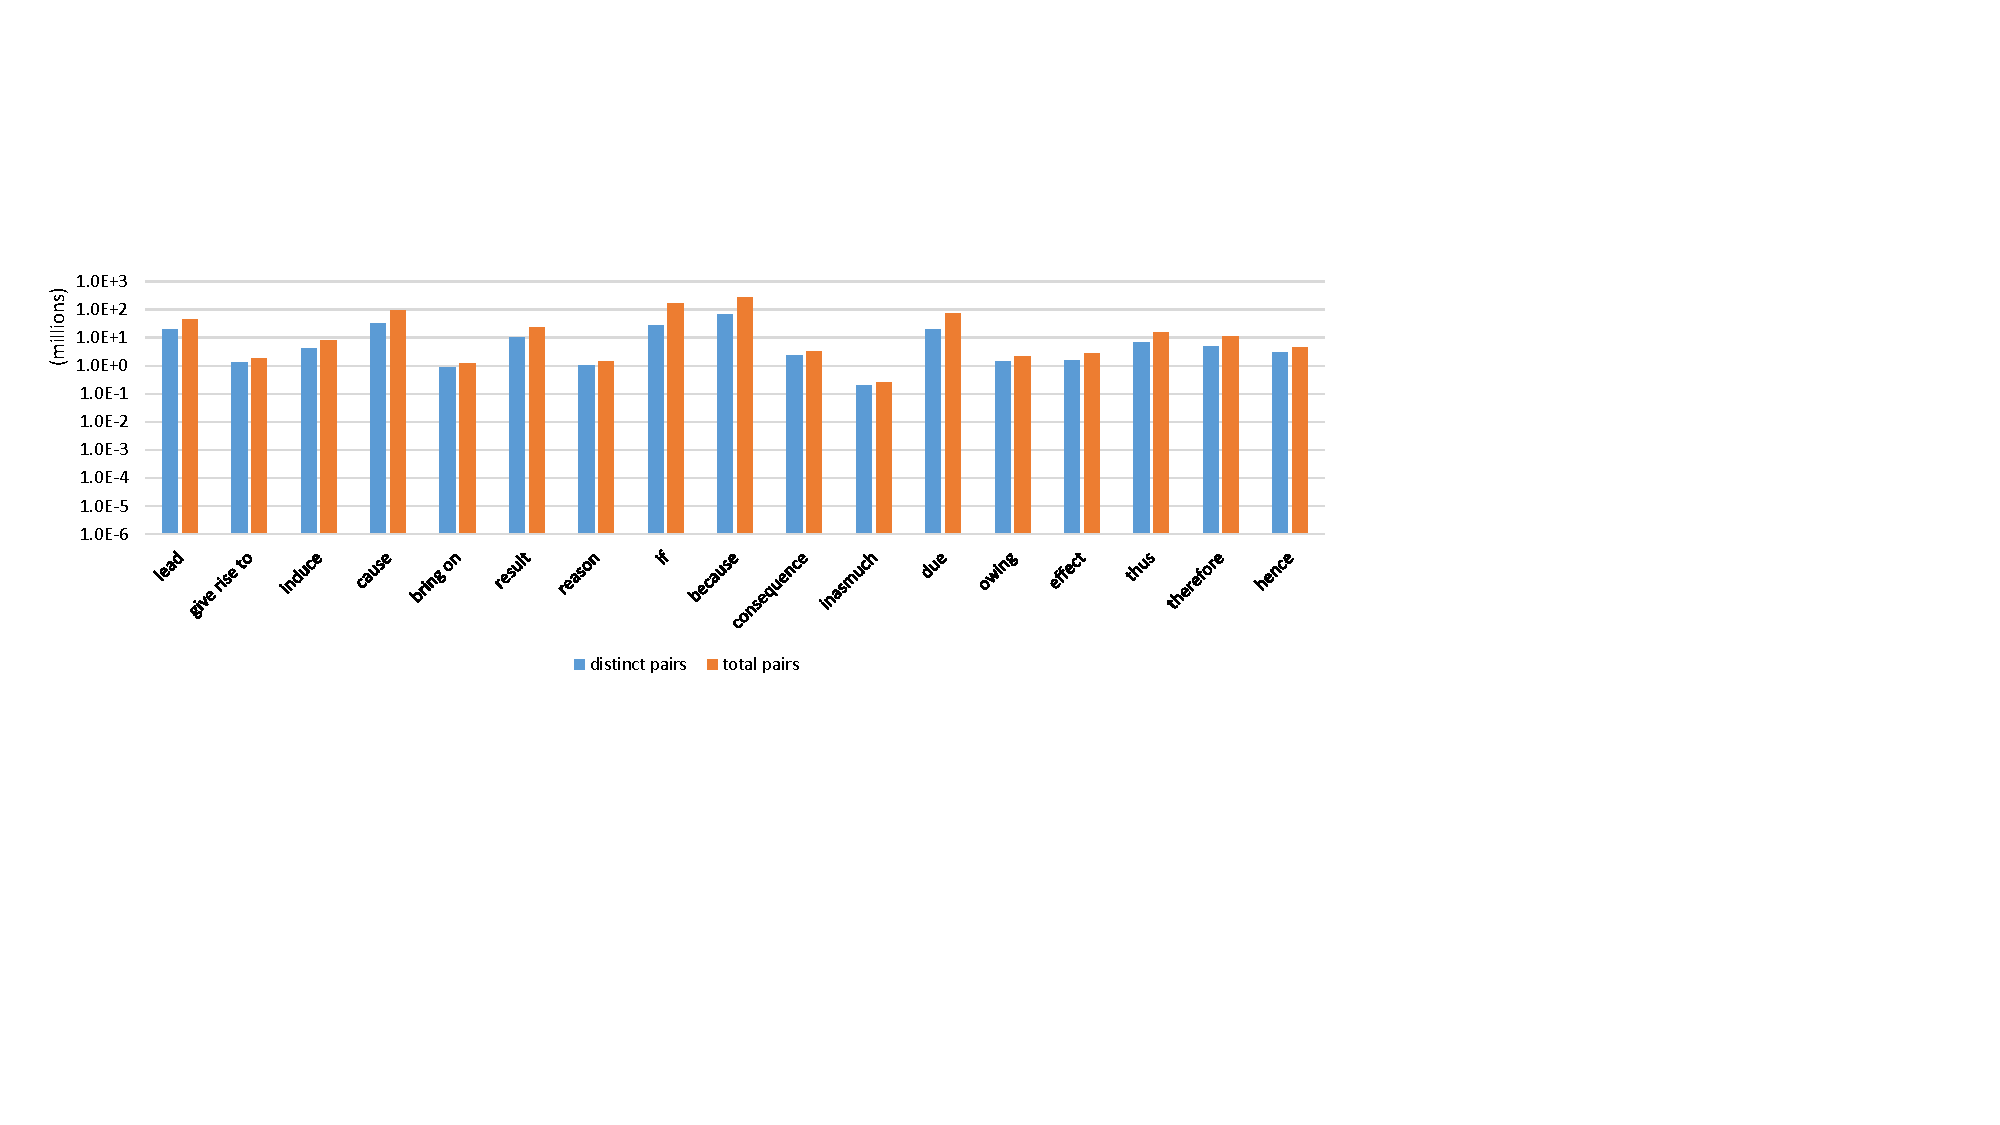
\includegraphics[width=2\columnwidth]{pattern.pdf}
\caption{COPA Results by varying corpus size of Gutenberg }

\label{fig:gu_pmi_1}
\end{figure}

\subsection{Causality Detection}
Another task is to investigate the following two research
questions on our proposed network, using data from ConceptNet4.

\begin{itemize}
\item {\bf RQ1:} For arbitrary event pair manually labeled as \emph{causal} (positive) or \emph{not causal} (negative), we investigate whether our proposed causality score clearly separates the two.
\item {\bf RQ2:} Inspired by COPA, we investigate positive and negative pair sharing the same premise, and investigate the accuracy of our selection of positive
alternative.
\end{itemize}

%More specifically,
%we use \emph{pseudo-disambiguation task} used in~\cite{Erk}.
%Intuitively, ConceptNet, being manually generated, is limited in coverage,
%but expected to be near-perfect in precision.
%In particular, we follow Erk to use
%near-perfect causal event pairs $(u,v)$ from ConceptNet as positive ground-truth
%for testing, and to pair $u$
%with another random instance $v$ as negative ground-truth instances.

%The task is then to choose more likely effect $u$ among $v$ and $v'$
%using our network.
%(We can report precision and recall, and high score
%indicates that we are as good as ConceptNet in detection, with XX times larger
%coverage.
%Maybe we can show some pairs we found, as in your EMNLP draft if we are proud.)


For {\bf RQ1,}
%We do two applications based on ConcpetNet to show both reasonable of our
%causality metric on global causal pairs (thought it is difficult to give a
%threshold for causal relationship identification task) and usefulness to select
%plausible cause/effect from multiple-choice.
we randomly  collect 100 positive and 100 negative ground truth of
causal Figure \ref{fig:conceptApp1} shows the causality score
($y$-axis) of 100 positive and negative pairs indexed randomly
($x$-axis). We can observe that scores of positive and negative
pairs are accurately distinguished by a linear function, such as
$y=10^{-2}$, indicated by the green line, with little overlap.

\begin{figure}[th]
\centering
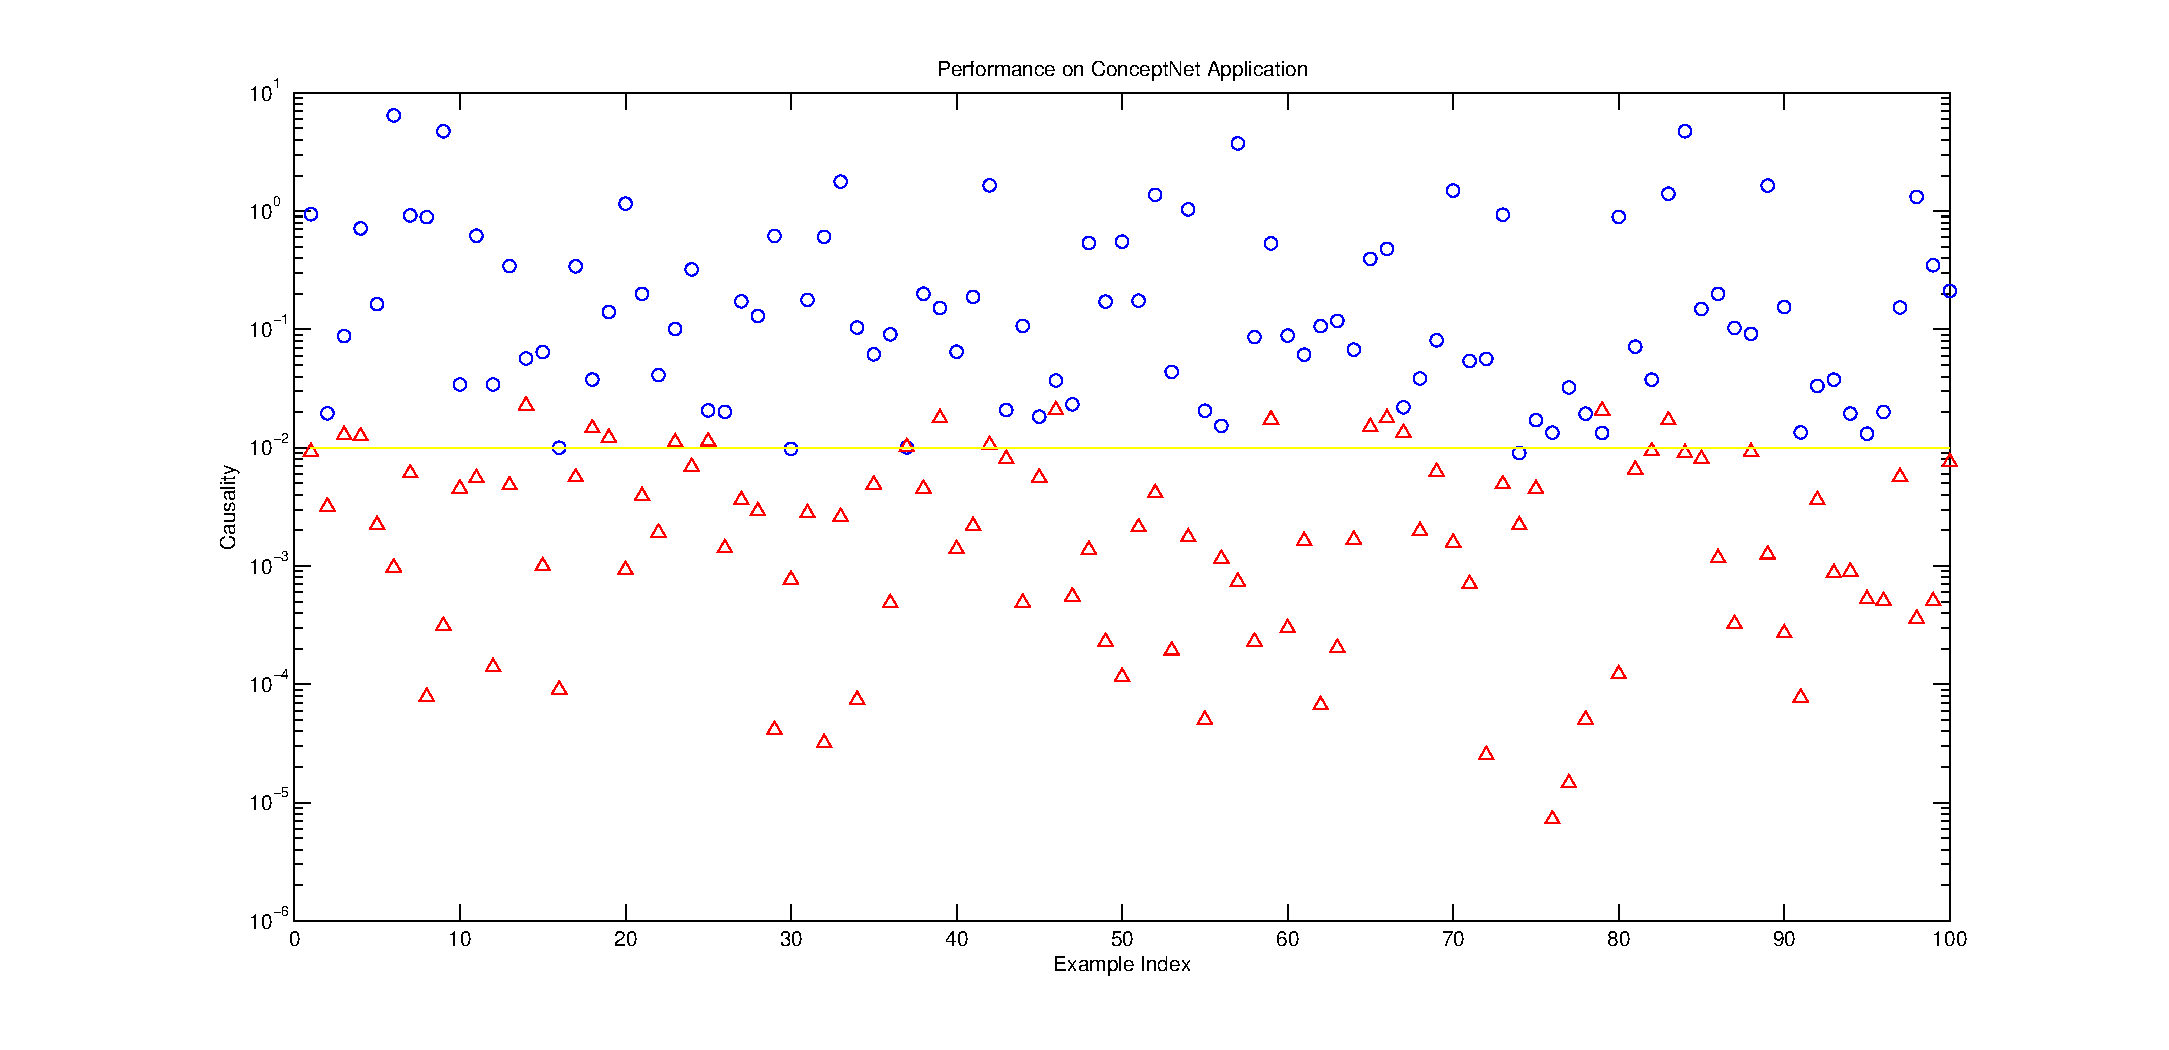
\epsfig{file=conceptApp1.eps, width=0.8\columnwidth}
\caption{Distinguishing causality on ConceptNet}
\label{fig:conceptApp1}
\end{figure}

For {\bf RQ2,} we test our network in a COPA-like setting
of classifying between positive and negative pairs sharing the same premise.
Due to sparsity of such pairs,
we use \emph{pseudo-disambiguation task} in~\cite{Erk}.
%Intuitively, ConceptNet, being manually generated, is limited in coverage,
%but expected to be near-perfect in precision.
In particular, we follow~\cite{Erk} to use
\emph{Causes} relationship
$(u,v)$ with positive votes, such that $u$ is the shared
premise and $v$ is a positive alternative.
We then generate a negative alternative by randomly selecting
$v'$ without \emph{Causes} relationship with $u$.
This approach is widely adopted in many tasks,
as a large scale test cases can be generated,
but as ConceptNet does not exhaustively label all possible causal relationships,
randomly selected $v'$ can be actually causal, or \emph{false negatives} exist.
In such situation, we removed the question involving such false negative,
and consequently obtained a dataset of 412 questions in which
259 looks for an effect while 153 looks for a cause. \tabref{tab:rq2}
shows the result using our framework with event detection outperforming
the other.

\begin{table}[th]
%\small
\centering
\caption{Result of ConceptNet RQ2}
\begin{tabular}{cc}
%\hline CausalNet w/ events & CausalNet w/o events   \\ \hline \hline
\hline
Methods & Accuracy(\%) \\
\hline
CausalNet w/o events & 78.4\%  \\
{\bf CausalNet w/ events} & {\bf 80.1\% }  \\
\hline
\end{tabular}
\label{tab:rq2}
\end{table}
